%%%%%%%%%%%%%%%%%%%%%%%%%%%%%%%%%%%%%%%%%%%%%%%%%%%%%%%%%%%%%%%%%%%%%
%% This is a (brief) model paper using the achemso class
%% The document class accepts keyval options, which should include
%% the target journal and optionally the manuscript type.
%%%%%%%%%%%%%%%%%%%%%%%%%%%%%%%%%%%%%%%%%%%%%%%%%%%%%%%%%%%%%%%%%%%%%
\documentclass[journal=jacsat,manuscript=article]{achemso}
\usepackage[german]{babel}
\SectionNumbersOn

%%%%%%%%%%%%%%%%%%%%%%%%%%%%%%%%%%%%%%%%%%%%%%%%%%%%%%%%%%%%%%%%%%%%%
%% Place any additional packages needed here.  Only include packages
%% which are essential, to avoid problems later.
%%%%%%%%%%%%%%%%%%%%%%%%%%%%%%%%%%%%%%%%%%%%%%%%%%%%%%%%%%%%%%%%%%%%%
\usepackage{notes2bib} % Formula subscripts using \ch{}
\usepackage[T1]{fontenc} % Use modern font encodings
\usepackage{hyperref}
\usepackage[hang]{footmisc}
\usepackage{lipsum}
\usepackage{multicol}
\usepackage{etoolbox,refcount}
\usepackage{graphicx}

\usepackage{mathtools}
\usepackage[export]{adjustbox}
\usepackage{babel,varioref}
\addto\extrasgerman{% page 5 of varioref's manual
  \renewcommand\reftextfaceafter{auf der n{\"a}chsten Seite}%
  \renewcommand\reftextafter {auf der n{\"a}chsten Seite}%
  \renewcommand\reftextfacebefore{auf der vorherigen Seite}%
  \renewcommand\reftextbefore {auf der vorherigen Seite}%
  \renewcommand\reftextcurrent {auf dieser Seite}%
}
\usepackage{listings}
\usepackage{float}
\usepackage{changepage}


\usepackage[
nochapters, % Turn off chapters since this is an article        
beramono, % Use the Bera Mono font for monospaced text (\texttt)
eulermath,% Use the Euler font for mathematics
pdfspacing, % Makes use of pdftex’ letter spacing capabilities via the microtype package
dottedtoc % Dotted lines leading to the page numbers in the table of contents
]{classicthesis} % The layout is based on the Classic Thesis style

\usepackage{arsclassica} % Modifies the Classic Thesis package

\usepackage[T1]{fontenc} % Use 8-bit encoding that has 256 glyphs

\usepackage[utf8]{inputenc} % Required for including letters with accents

\usepackage{graphicx} % Required for including images
\graphicspath{{Figures/}} % Set the default folder for images

\usepackage{enumitem} % Required for manipulating the whitespace between and within lists

\usepackage{lipsum} % Used for inserting dummy 'Lorem ipsum' text into the template

\usepackage{subcaption} % Required for creating figures with multiple parts (subfigures)

\usepackage{amsmath,amssymb,amsthm} % For including math equations, theorems, symbols, etc
\usepackage{cite}

%%%%%%%%%%%%%%%%%%%%%%%%%%%%%%%%%%%%%%%%%%%%%%%%%%%%%%%%%%%%%%%%%%%%%
%% If issues arise when submitting your manuscript, you may want to
%% un-comment the next line.  This provides information on the
%% version of every file you have used.
%%%%%%%%%%%%%%%%%%%%%%%%%%%%%%%%%%%%%%%%%%%%%%%%%%%%%%%%%%%%%%%%%%%%%
%%\listfiles

%%%%%%%%%%%%%%%%%%%%%%%%%%%%%%%%%%%%%%%%%%%%%%%%%%%%%%%%%%%%%%%%%%%%%
%% Place any additional macros here.  Please use \newcommand* where
%% possible, and avoid layout-changing macros (which are not used
%% when typesetting).
%%%%%%%%%%%%%%%%%%%%%%%%%%%%%%%%%%%%%%%%%%%%%%%%%%%%%%%%%%%%%%%%%%%%%
\newcommand*\mycommand[1]{\texttt{\emph{#1}}}

%%%%%%%%%%%%%%%%%%%%%%%%%%%%%%%%%%%%%%%%%%%%%%%%%%%%%%%%%%%%%%%%%%%%%
%% Meta-data block
%% ---------------
%% Each author should be given as a separate \author command.
%%
%% Corresponding authors should have an e-mail given after the author
%% name as an \email command. Phone and fax numbers can be given
%% using \phone and \fax, respectively; this information is optional.
%%
%% The affiliation of authors is given after the authors; each
%% \affiliation command applies to all preceding authors not already
%% assigned an affiliation.
%%
%% The affiliation takes an option argument for the short name.  This
%% will typically be something like "University of Somewhere".
%%
%% The \altaffiliation macro should be used for new address, etc.
%% On the other hand, \alsoaffiliation is used on a per author basis
%% when authors are associated with multiple institutions.
%%%%%%%%%%%%%%%%%%%%%%%%%%%%%%%%%%%%%%%%%%%%%%%%%%%%%%%%%%%%%%%%%%%%%
\author{Till Hildebrandt, inf102835}
\affiliation{University of Applied Sciences, Wedel}
\email{till.hildebrandt@gmail.com}


%%%%%%%%%%%%%%%%%%%%%%%%%%%%%%%%%%%%%%%%%%%%%%%%%%%%%%%%%%%%%%%%%%%%%
%% The document title should be given as usual. Some journals require
%% a running title from the author: this should be supplied as an
%% optional argument to \title.
%%%%%%%%%%%%%%%%%%%%%%%%%%%%%%%%%%%%%%%%%%%%%%%%%%%%%%%%%%%%%%%%%%%%%
\title[An \textsf{achemso} demo]
  {Anwendung neuronaler Netzer zur Verkehrsflussoptimierung}

%%%%%%%%%%%%%%%%%%%%%%%%%%%%%%%%%%%%%%%%%%%%%%%%%%%%%%%%%%%%%%%%%%%%%
%% Some journals require a list of abbreviations or keywords to be
%% supplied. These should be set up here, and will be printed after
%% the title and author information, if needed.
%%%%%%%%%%%%%%%%%%%%%%%%%%%%%%%%%%%%%%%%%%%%%%%%%%%%%%%%%%%%%%%%%%%%%
\abbreviations{IR,NMR,UV}
\keywords{FH-Wedel, Wedel, Mathematische Anwendungen Seminar, \LaTeX}


\setlength\footnotemargin{10pt}

\makeatletter
\def\@makefnmark{%
  \leavevmode
  \raise.9ex\hbox{\fontsize\sf@size\z@\normalfont\tiny\@thefnmark}}
\makeatother


\newcounter{countitems}
\newcounter{nextitemizecount}
\newcommand{\setupcountitems}{%
  \stepcounter{nextitemizecount}%
  \setcounter{countitems}{0}%
  \preto\item{\stepcounter{countitems}}%
}
\makeatletter
\newcommand{\computecountitems}{%
  \edef\@currentlabel{\number\c@countitems}%
  \label{countitems@\number\numexpr\value{nextitemizecount}-1\relax}%
}
\newcommand{\nextitemizecount}{%
  \getrefnumber{countitems@\number\c@nextitemizecount}%
}
\newcommand{\previtemizecount}{%
  \getrefnumber{countitems@\number\numexpr\value{nextitemizecount}-1\relax}%
}
\makeatother    
\newenvironment{AutoMultiColItemize}{%
\ifnumcomp{\nextitemizecount}{>}{3}{\begin{multicols}{2}}{}%
\setupcountitems\begin{itemize}}%
{\end{itemize}%
\unskip\computecountitems\ifnumcomp{\previtemizecount}{>}{3}{\end{multicols}}{}}

\graphicspath{ {media/} }

%%%%%%%%%%%%%%%%%%%%%%%%%%%%%%%%%%%%%%%%%%%%%%%%%%%%%%%%%%%%%%%%%%%%%
%% The manuscript does not need to include \maketitle, which is
%% executed automatically.
%%%%%%%%%%%%%%%%%%%%%%%%%%%%%%%%%%%%%%%%%%%%%%%%%%%%%%%%%%%%%%%%%%%%%
\begin{document}
\newpage

\tableofcontents

\newpage

%%%%%%%%%%%%%%%%%%%%%%%%%%%%%%%%%%%%%%%%%%%%%%%%%%%%%%%%%%%%%%%%%%%%%
%% Start the main part of the manuscript here.
%%%%%%%%%%%%%%%%%%%%%%%%%%%%%%%%%%%%%%%%%%%%%%%%%%%%%%%%%%%%%%%%%%%%%

\section{Einleitung}

Die folgende Ausarbeitung befasst sich mit der Optimierung von Ampelschaltungen in Verkehrsnetzen mithilfe neuronaler Netze, die sich den erweiterten Verkehrsmanagementsystemen (\textit{engl.} Advanced Traffic Management System
\footnote{
Wikipedia, \href{
https://en.wikipedia.org/wiki/Advanced\_Traffic\_Management\_System
}{
Advanced Traffic Management System,
} \\
https://en.wikipedia.org/wiki/Advanced\_Traffic\_Management\_System
}
)
zurordnen lässt. Zunächst wird das Problem beschrieben, die Motivation hergeleitet und die gegenwärtige Situation aufgezeigt. Anschließend werden neuronale Netze\footnote{Wikipedia, \href{https://de.wikipedia.org/wiki/K\%C3\%BCnstliches\_neuronales\_Netz}{Künstliches neuronales Netz,} \\ https://de.wikipedia.org/wiki/Künstliches\_neuronales\_Netz} in ihren Arten und Prinzipien sowie die Darstellung von Verkehrsnetzen in datenverarbeitenden Systemen behandelt. Diese Abschnitte bilden die Grundlage, um den Optimierungsansatz mit dem Hopefield-Modell\footnote{Wikipedia, \href{https://de.wikipedia.org/wiki/Hopfield-Netz}{Hopefield-Modell,} \\ https://de.wikipedia.org/wiki/Hopfield-Netz} genau vorzustellen und dessen Resultate mit denen anderer Lösungen zu vergleichen.

%TODO use this paragraph
Ziel ist es den Verkehrsfluss in Städten so zu optimieren, dass der Verkehr möglichst störungsfrei fließt. Ein besserer Verkehrsfluss bedeutet weniger Staus, heißt weniger Umweltbelastung und weniger Unfälle.

\subsection{Motivation}

Die aktuelle politische Situation im Kleinen, sowie der Klimawandel im Großen, treiben uns immer weiter dazu nach Möglichkeiten zu streben verantwortungsvoller mit unserer Umwelt umzugehen. Ein verbesserter Verkehrsfluss ermöglicht es nicht nur dem Reisenden (im Durchschnitt) schneller sein Ziel zu erreichen, er geht optimaler Weise auch einher mit weniger Standzeiten, weniger Motoren im Leerlauf und in energieaufwändigen Prozessen wie dem Anfahren, bei dem viel Energie aufgebracht wird und damit entsprechend viel CO\textsubscript{2} wie andere Schadstoffe produziert werden. Dies bedeutet auch weniger Verschleiß, was zu einem längeren Verwenden des Fahrzeugs und somit zu einer Reduktion der CO\textsubscript{2}-Bilanz\footnote{Wikipedia, \href{https://de.wikipedia.org/wiki/CO2-Bilanz}{CO\textsubscript{2}-Bilanz,} \\https://de.wikipedia.org/wiki/CO2-Bilanz} der Herstellung zugute kommt.

Zudem steigen die Anzahl zugelassener Fahrzeuge und das damit verbundene Verkehrsaufkommen seit Aufkommen des Automobils an fast stetig an\footnote{Statista, \href{https://www.statista.com/statistics/281134/number-of-vehicles-in-use-worldwide/}{\textit{engl.} Number of vehicles in use worldwide,} \\https://www.statista.com/statistics/281134/number-of-vehicles-in-use-worldwide/}\textsuperscript{,}\footnote{Statista, \href{https://de.statista.com/statistik/daten/studie/12131/umfrage/pkw-bestand-in-deutschland/}{PKW-Bestand in Deutschland,} \\https://de.statista.com/statistik/daten/studie/12131/umfrage/pkw-bestand-in-deutschland/}. Einzig die von der Bundesregierung ausgesprochene Abwrackprämie\footnote{Wikipedia, \href{https://de.wikipedia.org/wiki/Umweltpr\%C3\%A4mie}{Umweltprämie,} \\ https://de.wikipedia.org/wiki/Umweltprämie} im Jahr 2008 hat, zumindest in Deutschland, Wirkung gezeigt. Dennoch sind die Zahlen weiterhin am Steigen und somit ist auch künftig mit einer zunehmenden Belastung des Straßennetzes zu rechnen. Ein besserer Verkehrsfluss kann von einer höheren Effizienz der Auslastung der Kapazitäten der Straßen profitieren und dabei helfen Investitionen in infrastrukturelle Projekte im besten Fall zu vermeiden.

Abschließend besteht die sowohl emotionale als auch statistisch begründbare Vermutung, dass ein verbesserter Verkehrsfluss mit weniger und kürzeren Standzeiten zu einer angenehmeren Reise mit mehr Umsicht, Ruhe und weniger Unfällen führt. Statistisch ist eine Korrelation zwischen Fahrtzeit und der Wahrscheinlichkeit, dass ein Unfall eintritt zu erwarten.

%TODO hier schon die erste formel - keine sorge, so leicht bleibt es nicht
\[ P\textsubscript{strecke-kurz}(Unfall) < P\textsubscript{strecke-lang}(Unfall) \]

Es hat sich gezeigt, dass neuronale Netze ein gutes Werkzeug im Umgang mit Problemen sein können, die mit klassischen Verfahren nur schwer adressierbar sind. Dabei handelt es sich in der Regel um Probleme, die mit Daten umgehen, in denen es irgendeine Form an statistischen Zusammenhängen/Mustern gibt. So wurde mithilfe neuronaler Netze Software produziert, die eine künstliche Intelligenz für das Spiel Go\footnote{Wikipedia, \href{https://de.wikipedia.org/wiki/Go\_(Spiel)}{Go (Spiel)} https://de.wikipedia.org/wiki/Go\_(Spiel)}, bei dem der Mensch lange als ungeschlagen galt, realisiert oder eine, die eine Synchronisation von geschriebenem Text auf Mundbewegungen eines Videos bewerkstelligt\footnote{Joon Son Chung and Andrew Zisserman, Oxford University, \href{https://www.robots.ox.ac.uk/~vgg/publications/2016/Chung16a/chung16a.pdf}{Out of time: automated lip sync in the wild}}. Weitere Beispiele sind:

\begin{multicols}{2}
\begin{itemize}
    \item Schrifterkennung\footnote{Pythonprogramming, \href{https://pythonprogramming.net/image-recognition-python/}{Image Recorgnition with Python,}\\https://pythonprogramming.net/image-recognition-python/} %TODO AMAZON STORY ALINAS DAD
  \item Spracherkennung
  \item Gesichtserkennung
  \item Kaufempfehlungen
  \item Aktienkursanalysen
  \item Textübersetzungen
\end{itemize}
\end{multicols}

Bei dem hier behandelten Problem der Verkehrsflussoptimierung kann, ähnlich wie bei den oben genannten Probleme, ein starker statistischer Zusammenhang angenommen werden. In bestimmten Rhythmen fahren mehr oder weniger Menschen bestimmte Straßen in bestimme Richtungen. Der Verkehr ist dabei unterschiedlich dicht und schnell. Manche Strecken sind zu bestimmten Zeiten mehr ausgelastet, andere weniger. Klingt nach einem großartigen Anwendungsfall für neuronale Netze.

\subsection{Gegenwärtige Situation}

Derweil gibt es keine einheitlich angewandtes System zur Ampelsteuerung in Deutschland. Ampelphasen können fest definiert sein oder verkehrsabhängig gesetzt werden. Bei festen Definitionen werden die Zeiten in einem Signalzeitenplan\footnote{Wikipedia, \href{https://de.wikipedia.org/wiki/Signalzeitenplan}{Signalzeitenplan} https://de.wikipedia.org/wiki/Signalzeitenplan} festgehalten.

\begin{figure}[H]
    \centering
    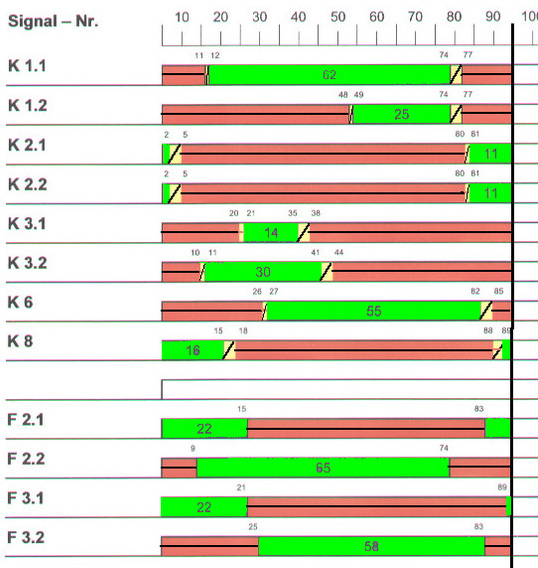
\includegraphics[width=0.7\textwidth]{signalzeitenplan_ausschnitt}
    \caption{Signalzeitenplan}
    \label{fig:signalzeitenplan}
\end{figure}

Auf der X-Achse befindet sich die Zeit in Sekunden, auf der Y-Achse die diskreten Werte der beteiligen Signalgeber. Rot- und Grünphasen sind in der jeweiligen Farbe dargestellt. Die übrigen Elemente entsprechen den beiden Gelbphasen Gelb und Rot/Gelb. Zu verstehen ist das Diagramm im Zeitfluss von links nach rechts. Rechts angekommen, geht es links wieder los.

Bei der verkehrsabhängigen Steuerung werden die einzelnen Verkehrsströme je nach Bedarf bedient. Sie funktioniert mithilfe vielerlei Technologien, so gibt es Induktionsschleifen und Bewegungsmelder, aber auch Videokameras unterstützen die Optimierung des Verkehrsflusses bei manchen Systemen. Vorwiegend handelt es sich dabei um Systeme, die an einzelnen Kreuzungen wirken und keinen größeren Bereich in Betracht ziehen. Sie sind zum Beispiel so konstruiert, dass alle ankommenden Fahrzeuge einer ankommenden Fahrzeugwelle die Kreuzung passieren können, die Ampelphasen werden dementsprechend angepasst. Dabei ist darauf zu achten, dass die Wartezeiten der anderen Verkehrsteilnehmer nicht unzumutbar werden oder ein Rückstau der Abbiegespuren entsteht, die die anderen Spuren einengt.

\begin{figure}[H]
    \centering
    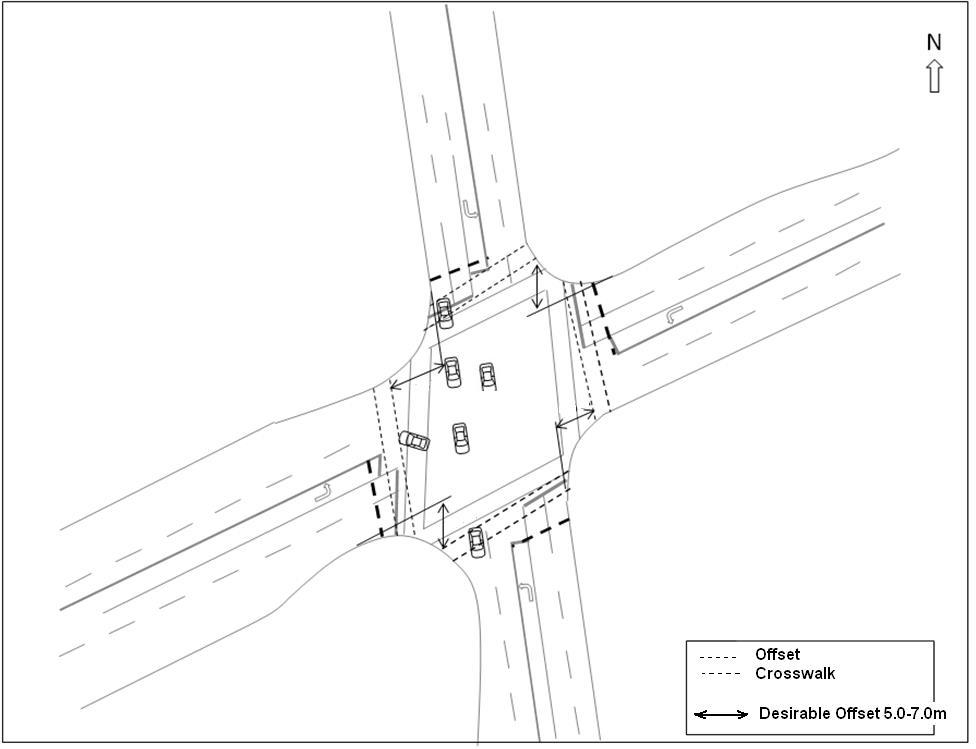
\includegraphics[width=0.7\textwidth]{offsetcrosswalk}
    \caption{Rückstau an einer Kreuzung}
    \label{fig:rueckstau}
\end{figure}

Daraus ergibt sich eine variable Umlaufzeit der Ampelphasen. Fest definierte Abläufe können zudem per Automatik zwischen verschiedenen Programmen wechseln, so kann auf verschiedene Verkehrsbelastungen (Berufs-, Tages- und Nachtverkehr usw.) reagiert werden.

Weitere Elemente des Straßenverkehrs, die den Verkehrsfluss direkt beeinflussen können, sind zum Beipiel Fußgängerampeln mit Anforderung oder einem Zebrastreifen. Es ist zwar wichtig, möchte man ein ganzheitliches System implementieren, diese Elemente zu betrachten, in dieser Ausarbeitung werden diese Elemente jedoch noch außen vorgelassen.

Der im Folgenden vorgestellte Optimierungsansatz mit dem Hopefield-Netzwerk betrachtet hingegen ein komplexes System an Straßen. Sozusagen einen Teilgraph des Verkehrsnetzes. Angewandt wurde das System im Zuge der Olympischen Spiele in Atlanta 1996\footnote{John F. G. and Khalid J. E., \href{https://www.aaai.org/Papers/Workshops/1993/WS-93-04/WS93-04-012.pdf}{Traffic Management Applications of Neural Networks,} \\https://www.aaai.org/Papers/Workshops/1993/WS-93-04/WS93-04-012.pdf}.

NOTES:
umlaufszeit 45 - 120 sek, Situation in HH
smart city 
atms
atlanta olympic
anforderung/bedarfsampeln

%\footnote{###NAME###, \href{###URL###}{###TITLE###,} \\###URL###}

\newpage


\newpage

\section{Neuronale Netze}

Neurnale Netze beziehen sich eigentlich auf biologische Nervenzentren. In der Informatik hat man nur das grundlegende Prinzip adaptiert und versucht Strukturen zu erzeugen, die anhand von Daten lernen können. Es wird nicht versucht ein \textit{echtes} Gehirn nachzuempfinden, in dem Metastrukturen auftreten, in denen bestimmte Bereiche bestimmte Aufgaben haben. An dem Bereich wird natürlich auch geforscht, ist aber Gegenstand der Computational NeuroscienceTODO.

\subsection{Grundprinzipichen}

Die nachfolgenden Ausführungen und Grafiken zum Schaffen eines grundlegenden Verständnisses für neuronale Netze, die hier verwendet werden, basieren im wesentlichen auf dem E-Book ``Neural Networks and Deep Learning''\footnote{Michael Nielsen, Neural Networks and Deep Learning.\newline(http://neuralnetworksanddeeplearning.com/index.html)}.

Im Rahmen des maschinellen Lernens stellen die neuronalen Netze einen elementaren Ansatz dar, der in vielen weiteren Modellen Verwendung findet. Neuronale Netze wie das maschinelle Lernen an sich stellen eine andere Herangehensweise dar, als die klassischer, deterministischer Algorithmen. Anstatt dem System eine eindeutige Abfolge von Anweisungen mitzuteilen, um eine konkrete Problemstellung zu lösen, wird ein Modell definiert und dieses mit verschiedenen Beispielen konfrontiert - die Beispiele sind dabei Tupel aus Eingangsgröße und erwarteter Ausgangsgröße. Die Dimensionen von Eingangs- und Ausgangsgröße können sich dabei gleich sein, müssen es aber nicht. So können als Eingabe Bilder dienen und als Ausgaben konkrete Klassen, um beispielsweise Hunde von Katzen unterscheiden zu können. TODO
Anstatt nun algorithmisch zu definieren, was einen Hund von einer Katze unterscheidet, wird es dem zuvor erstellten Modell überlassen, anhand der gegebenen Eingaben und erwarteten Ausgaben, eigenständig Regeln abzuleiten, um mit dessen Hilfe auch unbekannte Eingaben klassifizieren zu können.

Dieser Ansatz wird auch als \textit{Soft Computing} TODO bezeichnet.

\subsubsection{Perzeptron}

Als elementaren Bestandteil eines neuronalen Netzes dient das \textit{Perzeptron} - dieses stellt die kleinste Einheit eines neuronalen Netzes dar und wird auch als ``künstliches Neuron'' bezeichnet.

Grundsätzlich akzeptiert ein Neuron einen beliebig großen Input bestehend aus Features \textit{x1, x2, ..., xn} und berechnet daraus ein Ergebnis.

\begin{figure}[H]
    \centering
    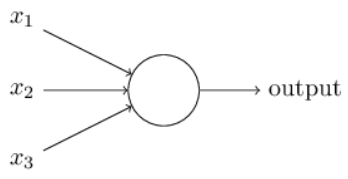
\includegraphics[width=0.5\textwidth]{docu_img_01}
    \caption{Perzeptron}
    \label{fig:perzeptron}
\end{figure}

Im gezeigten Bild ist beispielsweise ein Neuron dargestellt, das drei Inputgrößen akzeptiert und daraus einen Output produziert. Um den Output zu berechnen werden Gewichte (\textit{engl. weights}) eingeführt. Ob das Neuron 0 oder 1 als Output liefert, hängt dann davon ab, ob die gewichtete Summe der Eingangsgrößen einen zu definierenden Schwellwert überschreitet.

Dies kann anhand der nachfolgenden Formel verdeutlicht werden:

\begin{figure}[H]
    \centering
    \[ output =
      \begin{cases}
        0 \quad \text{if } \sum \omega_i x_i \leqslant \text{ threshold (Schwellwert)}\\
        1 \quad \text{if } \sum \omega_i x_i > \text{ threshold (Schwellwert)}
      \end{cases}
    \]
    \caption{Berechnung des Outputs.}
    \label{fig:neuron-three-way}
\end{figure}

Dies ist das grundlegende Modell. Grundsätzlich kann sich das Perzeptron auch als ein ``Entscheidungs-Unterstützer'' vorstellt werden, der eine Entscheidung trifft, in dem er konkrete Fakten mit einem bestimmten Gewicht versieht.

Das gezeigte Modell ist augenscheinlich sehr simpel und noch sehr weit von dem entfernt, was als ein neuronales Netz bezeichnet werden würde. Es ist allerdings ohne Weiteres denkbar, das gezeigte Model komplexer zu gestalten, indem mehrere Perzeptrons miteinander verknüpft werden, so dass beispielsweise das nachfolgende Netzwerk entstehen könnte:

\begin{figure}[H]
    \centering
    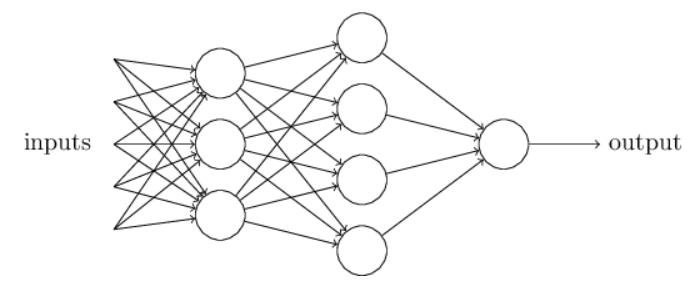
\includegraphics[width=0.5\textwidth]{docu_img_03}
    \caption{Mehrschichtiges neuronales Netz.}
    \label{fig:multi-layer-net}
\end{figure}

In Grafik\textsuperscript{\ref{fig:neuron-three-way}} wurde ein Schwellwert eingeführt, der überschritten werden muss, damit ein Perzeptron aktiviert wird. Um das Modell zu vereinheitlichen, kann der \textit{Bias} definiert werden, der den negativen Schwellwert darstellt. Durch diese Maßnahme kann die Aktivierungsfunktion des Perzeptrons dann geschrieben werden als:

\begin{figure}[H]
    \centering
    \[ output =
          \begin{dcases}
            0 \quad \text{if } \sum \omega \cdot x + b \leq 0 \\
            1 \quad \text{if } \sum \omega \cdot x + b > 0
          \end{dcases}
    \]
    \caption{Berechnung des Outputs bei Verwendung eines Bias.}
    \label{fig:bias-calculation}
\end{figure}

Inhaltlich kann der Bias als ein Maß verstanden werden, aus dem hervorgeht, wie \textit{leicht} ein Perzeptron aktiviert werden kann. Nimmt der Bias einen großen Wert an, so kann das Perzeptron einen Wert von 1 annehmen, auch wenn das Produkt aus den Gewichten und den Eingangsgrößen einen negativen Wert annimmt. Gleiches gilt selbstverständlich auch für einen kleinen Bias, der zur Folge hat, dass ein Perzeptron träger reagiert.

NOTE:
wiederholung gehirn menschlich lernen

\subsubsection{Sigmoid-Neuronen}

Eine Weiterentwicklung des zuvor vorgestellten Modells stellen Sigmoid-Neuronen dar. Diese Weiterentwicklung wird dann erforderlich, wenn das Anpassen der Gewichte - also letztlich das Lernen - betrachtet wird. Dabei ist das Ziel, dass eine kleine Anpassung eines Gewichts auch nur eine kleine Änderung des Outputs zur Folge hat. Das zuvor betrachtete Perzeptron ist lediglich in der Lage 0 oder 1 als Output zu liefern, so dass Änderungen an den Gewichten keine stetige Änderung des Outputs zur Folge haben, sondern folgenlos bleiben können bis irgendwann ein Sprung von 0 auf 1 oder umgekehrt stattfindet, was wiederum eine große Änderung darstellt.

Die Weiterentwicklung besteht nun in einer Verfeinerung der Aktivierungsfunktion. Anstatt eine Sprungfunktion\textsuperscript{\ref{fig:step-function}} zu verwenden, die lediglich 0 und 1 als Funktionswert annehmen kann, wird die Sigmoid Funktion\textsuperscript{\ref{fig:sigmoid-function}} eingeführt, die die folgende Form hat:

\begin{figure}[H]
    \centering
    \[ \sigma(z) \equiv
          \frac{1}{1+e^{-z}}
    \]
    \caption{Sigmoid-Funktion.}
    \label{fig:sigmoid}
\end{figure}

Der entscheidende Unterschied kann an den beiden nachfolgenden Grafiken verdeutlicht werden, die jeweils die Kurve der entsprechenden Funktion darstellen:

\captionsetup[subfigure]{labelformat=empty, labelsep=none}
\begin{figure}[H]
    \centering
    \begin{subfigure}{0.45\textwidth}
		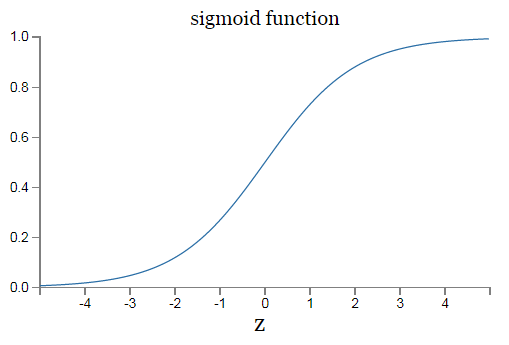
\includegraphics[width=0.9\textwidth]{docu_img_06}
		\caption{\tiny{Sigmoid Funktion.}}
		\label{fig:sigmoid-function}
	\end{subfigure}
    \begin{subfigure}{0.45\textwidth}
		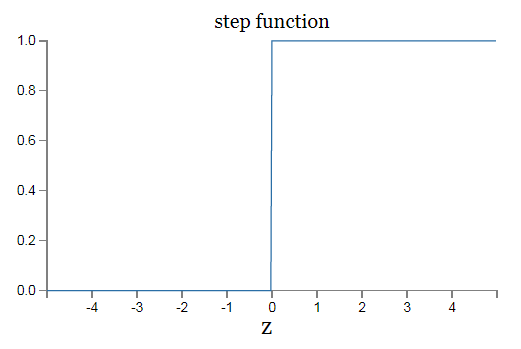
\includegraphics[width=0.9\textwidth]{docu_img_07}
		\caption{\tiny{Step Funktion.}}
		\label{fig:step-function}
	\end{subfigure}

    \caption{Vergleich der Aktivierungsfunktionen \textit{Sigmoid} und \textit{Step-Funktion}}
    \label{fig:activation-functions}
\end{figure}

\subsubsection{Architektur neuronaler Netze}

Mit diesen Bestandteilen als Ausgangspunkt können nun tatsächlich konkretere Neuronale Netze und deren Architekturen eingeführt werden. Neuronale Netze bestehen üblicherweise aus mehreren Schichten, den \textit{Layern}. Diese lassen sich grundsätzlich in drei Kategorien aufteilen: Input, Hidden und Output. Neuronale Netze beinhalten für gewöhnlich ein Input-Layer und ein Output-Layer sowie dazwischen beliebig viele Hidden-Layer. Die Form der Input- und Output-Layer ist dabei sehr naheliegend: das Input-Layer hat die gleiche Struktur wie die des Inputs und das Output-Layer hat entsprechend die gleiche Struktur wie der Output.

Angenommen es sollen Bilder der Größe 28 \(\times\) 28 Pixel klassifiziert werden und es gibt 10 mögliche Klassen, dann besteht das Input-Layer aus 28 \(\times\) 28 = 784 Neuronen und das Output-Layer aus 10 Neuronen.

Lediglich der Bereich zwischen Input- und Output-Layer - die Hidden-Layer - lässt sich nicht ohne Weiteres aus dem Input oder dem Output ableiten. Es gibt lediglich Heuristiken, die beim Design der Hidden-Layer angewandt werden können, allerdings keine konkreten Regeln, die befolgt werden müssen. Diese Struktur kann anhand des nachfolgenden Bilds verdeutlicht werden, bei dem - um die Übersichtlichkeit zu wahren - das Input-Layer etwas komprimiert dargestellt wird:

NOTES:
pyton tutorial uh - > softcomputing

\begin{figure}[H]
    \centering
    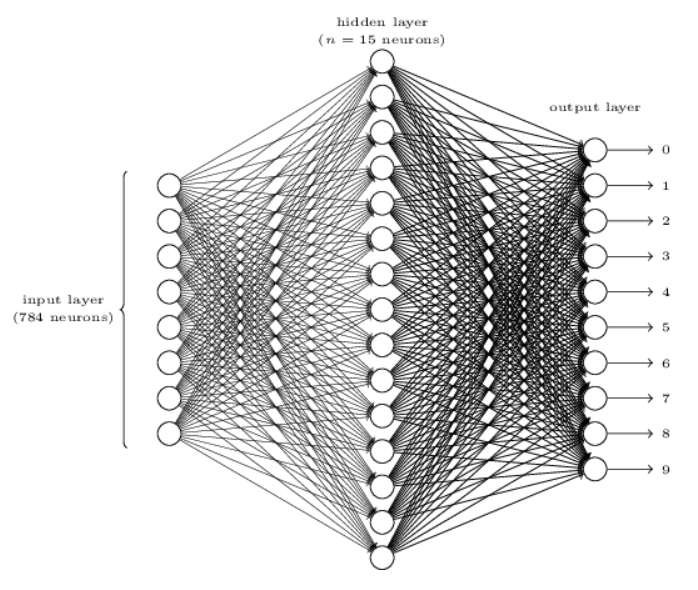
\includegraphics[width=0.9\textwidth]{docu_img_08}
    \caption{Hidden-Layer Darstellung.}
    \label{fig:hidden-layers}
\end{figure}

\subsection{Lernen - Das Anpassen der Gewichte}

Das Lernen stellt den zentralen Ansatz von neuronalen Netzes dar. Eng im Zusammenhang mit dem Lernen steht eine
Kosten-Funktion, die häufig auch als Verlust-Funktion bezeichnet werden kann. Diese stellt letztlich den Fehler zwischen
dem Erwartungswert und dem tatsächlichen Wert, den das neuronale Netz berechnet, dar. Mathematisch betrachtet ist das
grundlegende Prinzip des Lernens, diese Funktion zu minimieren, also zu gewährleisten, dass die Abweichungen zwischen
Erwartungswert und tatsächlichem Wert möglichst gering sind. Es sind grundsätzlich viele verschiedene Verlust-Funktionen
denkbar, eine, die jedoch eine breite Verwendeung findet, ist die quadratische Kosten-Funktion - auch als \textit{mean squared
error} (MSE) bezeichnet.

\begin{figure}[H]
    \centering
    \[ C(w, b) \equiv
          \frac{1}{2n}\displaystyle\sum_{x}{\parallel y(x) - a\parallel^2}
    \]
    \caption{Mean Squared Error (MSE).}
    \label{fig:learn-function}
\end{figure}

Dabei beschreiben \textit{w} und \textit{b} die Gewichte bzw. die Bias des neuronalen Netzes und \textit{n} stellt die Anzahl der Trainingsdaten
dar. Der Vektor a beschreibt den Output des Netzes und \textit{\(y(x)\)} stellt den Erwartungswert zu einem Input \textit{x} dar.
Das Ziel besteht nun darin, die Gewichte und Bias so zu manipulieren, dass die gezeigte Funktion einen möglichst kleinen
Wert annimmt.







--
Wie Neuronen funktionieren
Die Arbeitsweise ist erstaunlich einfach:
Immer wenn die Summe der Eingangssignale einen bestimmten Schwellenwert überschreitet,
sendet die Zelle ein Ausgangssignal.
Bleibt die Eingangserregung unter der Grenze, reagiert die Zelle nicht.
Am Ende der axonalen Verzweigungen stellt eine besondere Struktur, die Synapse,
den Kontakt zu anderen Neuronen her.
Die meisten Synapsen funktionieren so:
Je stärker die Erregung im Axon, desto mehr Moleküle einer Überträgersubstanz
schüttet die Synapse aus. Der Überträgerstoff (Neurotransmitter) wandert zur Zielzelle.
Manche Neurotransmitter erhöhen die elektrische Erregung der "angefunkten" Zelle,
andere hemmen sie. 

Die Netzwerke der Erinnerungf_artificial_neural_networks
Das Netzwerk der Neuronen in der Großhirnrinde (wegen ihrer Form auch „Pyramidenzellen“)
ist im Gegensatz zu einem Computer nicht nach einem detaillierten Plan geknüpft,
sondern weitgehend zufällig organisiert.
Sind miteinander verbundene Zellen gemeinsam aktiv, verstärken sich die Synapsen.
Demnach aktiviert das Lernen immer wieder eine Anzahl miteinander verknüpfter
Pyramidenzellen. Deren Verbindung verstärkt sich nach und nach,
„neuronale Netzwerke“ entstehen.
Je öfter sich der synaptische Lernprozess wiederholt, desto leichter
lässt sich dieses „Netzwerk“ aktivieren. 
--

\subsection{Arten und Anwendungsgebiete}

es gibt sie in allen formen und farben. nns zu listen, wäre ein akt der unmöglcihekit. 
im netz finden sich links wie:

The mostly complete chart of Neural Networks, explained
https://towardsdatascience.com/the-mostly-complete-chart-of-neural-networks-explained-3fb6f2367464

und
liste auf wikipedia
%https://en.wikipedia.org/wiki/Types\_of\_artificial\_neural\_networks


\subsection{Überwachtes und Unüberwachtes Lernen}
Lorem ipsum dolor sit amet, consetetur sadipscing elitr, sed diam nonumy eirmod tempor invidunt ut labore et dolore magna aliquyam erat, sed diam voluptua. At vero eos et accusam et justo duo dolores et ea rebum. Stet clita kasd gubergren, no sea takimata sanctus est Lorem ipsum dolor sit amet. Lorem ipsum dolor sit amet, consetetur sadipscing elitr, sed diam nonumy eirmod tempor invidunt ut labore et dolore magna aliquyam erat, sed diam voluptua. At vero eos et accusam et justo duo dolores et ea rebum. Stet clita kasd gubergren, no sea takimata sanctus est Lorem ipsum dolor sit amet.


\newpage



%%%%%%%%%%%%%%%%%%%%%%%%%%%%%%%%%%%%%%%%%%%%%%%%%%%%%%%%%%%%%%%%%%%%%
%% Start the main part of the manuscript here.
%%%%%%%%%%%%%%%%%%%%%%%%%%%%%%%%%%%%%%%%%%%%%%%%%%%%%%%%%%%%%%%%%%%%%
\section*{Verkehrsmodelle (5-6 Minuten)}
die fragestellung, wie lassen sich verkehrsnetze abbilden?

In the traffic flow problem, there are two classes of models: Macro- scopic, which is concerned with average behavior, such as traffic den- sity, average speed and module area, and a second class of models based on individual behavior referred to as microscopic models. The latter is classified into different types. The most famous one is the Car-Following models [6, 17, 57], where the driver adjusts his or her acceleration according to the conditions in front
-- ungern
Another type of microscopic models are the Cellular Automata or vehicle hopping which differs from Car-Following in that it is a fully discrete model. It considers the road as a string of cells which are either empty or occupied by one vehicle. One such model is the Stochastic Traffic Cellular Automata, given in [75].
--
, microscopic approaches are computationally expensive,as each car has an ODE to be solved at each time step, and as the number of cars increases, so does the size of the system to be solved.
On the other hand, the macroscopic models are com- putationally less expensive because they have fewer design details in terms of interaction among vehicles and between vehicles and their environment.

\subsection*{Mikroskopische Modelle}
In contrast to macroscopic models, microscopic traffic flow models simulate single vehicle-driver units, so the dynamic variables of the models represent microscopic properties like the position and velocity of single vehicles.

We present the well known car-following microscopic traffic flow model. In [93], a 2-D version of this model was used for pedestrian flow in 2-D space. To derive the 1-D model, first assume cars can not pass each other. Then the idea is that a car in 1-D can move and accelerate forward based on two parameters; the headway distance between the current car and the one in front, and their speed differ- ence. Hence, it is called following, where a car from behind follows the one in front, and this is the anisotropic property. This property is also desirable in macroscopic models, since it reflects the actual observed behavior of traffic flow [23].
Suppose the nth car location is xn(t), then the nonlinear model is given by

The acceleration of the current car depends on the front car speed and location, c is the sensitivity parameter. Integrating the above yields
 (2.2) Since by the definition of the density (number of cars per unit area)

and the integration constant dn is chosen such that at jam density
pm, the velocity is zero. Then for steady-state we get

pm
We see that for p -> 0 we get in trouble, but from observations in low traffic densities, car speed is the maximum allowed speed, hence we can assume v = vmax, which is the maximum allowed speed.

\subsection*{Makroskopische Modelle}
Traffic Flow Theory
In this section we will cover the vehicle traffic flow fundamentals for the macroscopic modeling approach. The relation between density, velocity and flow is presented for traffic flow. Then we derive the conservation of vehicles, which is the main governing equation for scalar macroscopic traffic models. Finally, the velocity–density func- tions that makes the conservation equation a function of only one variable (density) are given.
2.4.1 Flow
In this section, we will illustrate the close relationship between the three variables: density, velocity and traffic flow. Suppose there is a road with cars moving with constant velocity v0, and constant density p0 such that the distance between the cars is also constant as shown in the Fig. 2.1a. Now let an observer measure the number of cars per unit time tau that pass him (i.e. traffic flow f). In tau time, each car has moved v0tau distance, and hence the number of cars that pass the observer in tau time is the number of cars in v0tau distance, see Fig. 2.1b.
Since the density p0 is the number of cars per unit area and there is v0tau distance, then the traffic flow is given by
f = p0v0 (2.5) This is the same equation as in the time varying case, i.e.,
f (p, v) = p(x, t)v(x, t).

Fig. 2.1. (a) Constant flow of cars; (b) Distance traveled in tau hours for a single car
To show this, consider the number of cars that pass point x = x0 in a very small time Dt. In this period of time the cars have not moved far and hence v(x, t), and p(x, t) can be approximated by their constant values at x = x0 and t = t0. Then, the number of cars passing the observer occupy a short distance, and they are approximately equal to p(x, t)v(x, t)t, where the traffic flow is given by (2.6).

2.4.2 Conservation Law
The models for traffic, whether they are one-equation or system of equations, are based on the physical principle of conservation. When physical quantities remain the same during some process, these quan- tities are said to be conserved. Putting this principle into a mathe- matical representation will make it possible to predict the densities and velocities patterns at future time. In our case, the number of cars in a segment of a highway [x1,x2] are our physical quantities, and the process is to keep them fixed (i.e., the number of cars coming in equals the number of cars going out of the segment). The deriva- tion of the conservation law is given in [26, 37], and it is presented here for completion. Consider a stretch of highway on which cars are

\newpage

%%%%%%%%%%%%%%%%%%%%%%%%%%%%%%%%%%%%%%%%%%%%%%%%%%%%%%%%%%%%%%%%%%%%%
%% Start the main part of the manuscript here.
%%%%%%%%%%%%%%%%%%%%%%%%%%%%%%%%%%%%%%%%%%%%%%%%%%%%%%%%%%%%%%%%%%%%%
\section*{Das Hopfield Netzwerk und der Verkehrsfluss (15-20 Minuten)}
Lorem ipsum dolor sit amet, consetetur sadipscing elitr, sed diam nonumy eirmod tempor invidunt ut labore et dolore magna aliquyam erat, sed diam voluptua. At vero eos et accusam et justo duo dolores et ea rebum. Stet clita kasd gubergren, no sea takimata sanctus est Lorem ipsum dolor sit amet. Lorem ipsum dolor sit amet, consetetur sadipscing elitr, sed diam nonumy eirmod tempor invidunt ut labore et dolore magna aliquyam erat, sed diam voluptua. At vero eos et accusam et justo duo dolores et ea rebum. Stet clita kasd gubergren, no sea takimata sanctus est Lorem ipsum dolor sit amet.

\subsection*{Ampelschaltung}
Lorem ipsum dolor sit amet, consetetur sadipscing elitr, sed diam nonumy eirmod tempor invidunt ut labore et dolore magna aliquyam erat, sed diam voluptua. At vero eos et accusam et justo duo dolores et ea rebum. Stet clita kasd gubergren, no sea takimata sanctus est Lorem ipsum dolor sit amet. Lorem ipsum dolor sit amet, consetetur sadipscing elitr, sed diam nonumy eirmod tempor invidunt ut labore et dolore magna aliquyam erat, sed diam voluptua. At vero eos et accusam et justo duo dolores et ea rebum. Stet clita kasd gubergren, no sea takimata sanctus est Lorem ipsum dolor sit amet.

\subsection*{Hopfield Modell}
Lorem ipsum dolor sit amet, consetetur sadipscing elitr, sed diam nonumy eirmod tempor invidunt ut labore et dolore magna aliquyam erat, sed diam voluptua. At vero eos et accusam et justo duo dolores et ea rebum. Stet clita kasd gubergren, no sea takimata sanctus est Lorem ipsum dolor sit amet. Lorem ipsum dolor sit amet, consetetur sadipscing elitr, sed diam nonumy eirmod tempor invidunt ut labore et dolore magna aliquyam erat, sed diam voluptua. At vero eos et accusam et justo duo dolores et ea rebum. Stet clita kasd gubergren, no sea takimata sanctus est Lorem ipsum dolor sit amet.


\newpage


%%%%%%%%%%%%%%%%%%%%%%%%%%%%%%%%%%%%%%%%%%%%%%%%%%%%%%%%%%%%%%%%%%%%%
%% Start the main part of the manuscript here.
%%%%%%%%%%%%%%%%%%%%%%%%%%%%%%%%%%%%%%%%%%%%%%%%%%%%%%%%%%%%%%%%%%%%%
\section*{Resultate (5-6 Minuten)}
Lorem ipsum dolor sit amet, consetetur sadipscing elitr, sed diam nonumy eirmod tempor invidunt ut labore et dolore magna aliquyam erat, sed diam voluptua. At vero eos et accusam et justo duo dolores et ea rebum. Stet clita kasd gubergren, no sea takimata sanctus est Lorem ipsum dolor sit amet. Lorem ipsum dolor sit amet, consetetur sadipscing elitr, sed diam nonumy eirmod tempor invidunt ut labore et dolore magna aliquyam erat, sed diam voluptua. At vero eos et accusam et justo duo dolores et ea rebum. Stet clita kasd gubergren, no sea takimata sanctus est Lorem ipsum dolor sit amet.

\section*{Fazit (5-6 Minuten)}
Lorem ipsum dolor sit amet, consetetur sadipscing elitr, sed diam nonumy eirmod tempor invidunt ut labore et dolore magna aliquyam erat, sed diam voluptua. At vero eos et accusam et justo duo dolores et ea rebum. Stet clita kasd gubergren, no sea takimata sanctus est Lorem ipsum dolor sit amet. Lorem ipsum dolor sit amet, consetetur sadipscing elitr, sed diam nonumy eirmod tempor invidunt ut labore et dolore magna aliquyam erat, sed diam voluptua. At vero eos et accusam et justo duo dolores et ea rebum. Stet clita kasd gubergren, no sea takimata sanctus est Lorem ipsum dolor sit amet.
technologische weiterentwicklung autonomes fahren


\newpage

\listoffigures

\newpage

\listoftables

%%%%%%%%%%%%%%%%%%%%%%%%%%%%%%%%%%%%%%%%%%%%%%%%%%%%%%%%%%%%%%%%%%%%%
%% The appropriate \bibliography command should be placed here.
%% Notice that the class file automatically sets \bibliographystyle
%% and also names the section correctly.
%%%%%%%%%%%%%%%%%%%%%%%%%%%%%%%%%%%%%%%%%%%%%%%%%%%%%%%%%%%%%%%%%%%%%
\bibliography{achemso-demo}

\end{document}
